% Draft manuscript. Compiled with a generic two-column article layout that
% approximates the AAAI camera geometry; swap in aaai26.sty for submission
% (section structure and lengths are compatible).
\documentclass[10pt,twocolumn]{article}
\usepackage[letterpaper,margin=0.75in,columnsep=0.25in]{geometry}
\usepackage{times}
\usepackage{graphicx}
\usepackage{booktabs}
\usepackage{amsmath}
\usepackage{multirow}
\usepackage[numbers,sort&compress]{natbib}
\usepackage{caption}
\captionsetup{font=small,labelfont=bf}
\setlength{\bibsep}{2pt}

\title{\bf How Much Communication Does Deep Mutual Learning Need?}
\author{Anonymous submission}
\date{}

\begin{document}
\maketitle

\begin{abstract}
Deep Mutual Learning (DML) trains a cohort of neural networks that improve one
another by mimicking each other's predictions. In its standard form the cohort
is densely coupled---every network distills from every other---so the
communication cost is quadratic in the cohort size: $\Theta(K^2)$ pairwise
imitation terms per round. We show this cost is almost entirely unnecessary.
Coupling each network to a single peer per round, re-paired at random, reduces
communication from quadratic to linear---$\Theta(K)$---yet recovers almost the
entire benefit of dense DML---consistently across CIFAR-100 and CIFAR-10,
homogeneous and heterogeneous cohorts, and clean and heavily label-corrupted
training.
Under a matched communication budget the advantage is decisive: allotted only
the bandwidth a single-partner cohort spends to converge ($\approx$72\% test
accuracy), dense DML reaches just $\approx$41\%---a 31-point gap on the
accuracy--communication frontier. A systematic ablation of the communication
mechanism---random sparse pairing, maximum-weight matching on several
disagreement- and accuracy-based signals, variable per-round degree, fixed
communication graphs, and averaged-versus-per-peer targets---shows that the
benefit is governed by \emph{degree}, the number of peers each network imitates
per round, plus a small, quickly-saturating local-pool effect: no selection
rule beats random pairing, and graph structure is inert. Structure re-enters
on the \emph{failure} side: when a cohort member degrades, the communication
graph governs how damage propagates---contagious collapse in fragile cohorts,
and a measured one-hop, healing, quarantinable dose--response law in robust
ones. Together these results recast mutual learning as an inherently
communication-efficient procedure whose operative axis is degree, and whose
fault-tolerance depends on the structure that its accuracy does not.
\end{abstract}

\section{Introduction}

Deep Mutual Learning \citep{zhang2018deep} trains $K$ networks together, each
minimizing its supervised loss plus a KL term pulling its predictive
distribution toward each peer's. The protocol is symmetric and dense: every
model imitates every other, so each round computes $\Theta(K^2)$ pairwise
imitation terms and, in any distributed realization, exchanges $\Theta(K^2)$
prediction messages. Two assumptions are implicit in this design: that the
dense coupling is worth its quadratic price, and---an intuition shared by a
long line of peer-learning and matchmaking work---that choosing \emph{which}
peers a model imitates should matter.

We test both assumptions with a replication-gated experimental program
(385 runs; every comparison paired at the per-model level by shared
initialization and batch order) and find both essentially false:

\textbf{1. The degree law.} The benefit of mutual learning is governed by the
number of peers each model imitates per round (its \emph{degree}), and almost
nothing else. One random partner per round retains 82--90\% of the dense
benefit at $1/(K{-}1)$ of the communication; the dense premium is
$+0.3$--$0.5$ points at $7$--$11\times$ the traffic. At equal communication
budget the comparison is not close: sparse reaches 71.7\% where dense has
attained 40.6\% (Fig.~\ref{fig:pareto}).

\textbf{2. Nothing else matters (for accuracy).} Partner selection by
maximum-weight matching on four measured signals ties random pairing;
rotating and frozen partners tie; averaged and per-peer targets tie; ring,
prism, and expander graphs of equal degree tie; and fully \emph{disconnected}
sub-cohorts match their connected counterparts up to a small local-pool
effect that saturates by pool size $\approx 3$
(Table~\ref{tab:nulls}).

\textbf{3. The conversion mechanism.} The benefit is largest exactly where
individuals are weak but the cohort is collectively strong. Under 40\% label
noise, individually-collapsed models (50.6\%) sit inside an ensemble that
still attains 64.8\%; coupling of any structure converts that collective
knowledge into individual competence ($+7.7$ to $+8.6$ points), and degree~1
captures 90\% of the conversion (Fig.~\ref{fig:conversion}).

\textbf{4. Structure governs failure, not learning.} The same links that
carry the (structure-indifferent) benefit carry damage when a member
degrades. In fragile cohorts a single spontaneously-collapsed model triggers
graph-borne cascades---full-cohort collapse in 40\% of connected runs, never
across a disconnection boundary, with wave speed set by graph mixing. In
robust cohorts, a controlled ``dead teacher'' implant yields a clean
dose--response law: about $-1$ point for its direct neighbors, nothing beyond
one hop, exact quarantine under partition, zero induced deaths---and the
damage \emph{heals} within 10--30 epochs once exposure stops
(Figs.~\ref{fig:contagion},~\ref{fig:damage}).

The practical upshot inverts the usual accounting. Sparse mutual learning is
not a cheap approximation to dense DML; on the axes that matter in
deployment---communication and fault-tolerance---it is the better design,
surrendering only a fraction of a point of accuracy.

\section{Related Work}

\textbf{Mutual learning and codistillation.} DML \citep{zhang2018deep}
established dense online mutual distillation; codistillation
\citep{anil2018large} showed prediction-exchange distillation works at
datacenter scale and noted its communication appeal. Neither work ablates the
communication structure itself; our contribution is the systematic
program---degree, selection, rotation, topology, connectivity---showing that
of all these axes only degree (plus a saturating pool term) is active, and
the accompanying failure-channel analysis, which has no analogue in either
line. Offline distillation of an ensemble into a student
\citep{hinton2015distilling} is the two-phase limit of this family.

\textbf{Decentralized SGD.} Gossip-based training
\citep{lian2017can,ying2021exponential} studies parameter averaging over
graphs, where topology enters convergence bounds through the spectral gap yet
often matters less in practice than theory suggests. Our setting exchanges
\emph{predictions}, not parameters: models remain distinct functions, and no
consensus in weight space is sought. The observed inertness of topology has,
we argue, a sharper explanation here: with fully shared data there is no
knowledge gradient for the graph to transport (\S\ref{sec:nulls}).

\textbf{Robustness in collaborative learning.} Byzantine-robust aggregation
\citep{blanchard2017machine} treats adversarial gradient suppliers with
worst-case defenses. Our failure analysis is complementary and, to our
knowledge, new in kind: the \emph{epidemiology} of a benign protocol with a
degraded member---propagation, dose--response, recovery, and quarantine---
rather than attack and defense. The damage mechanism itself connects to
confidence penalties \citep{pereyra2017regularizing,szegedy2016rethinking}:
a collapsed model teaches the uniform distribution, and imitating it is
entropy regularization at toxic weight.

\textbf{Peer-learning societies.} Resource-constrained knowledge-diffusion
processes \citep{beikihassan2023resource} study the complementary regime, in
which knowledge is \emph{localized} (a rationed oracle) and the interaction
structure is decisive. Read together with our results, the two regimes
suggest a single organizing principle: communication structure couples to
knowledge gradients---inert when knowledge is ubiquitous (this paper),
decisive when it is localized (theirs). Classical social-learning theory
makes a matching observation about correlation destroying the wisdom of
crowds \citep{golub2010naive}, which reappears here as the ensemble cost of
coupling.

\section{Experimental Setup}
\label{sec:setup}

\textbf{Cohorts and training.} We train cohorts of $K\in\{2,\dots,12\}$
CIFAR-100 classifiers (ResNet-32; heterogeneous cells mix WRN-28-10
\citep{zagoruyko2016wide} and MobileNet \citep{howard2017mobilenets};
a weak-learner probe uses a LeNet-5 variant) with the DML paper's recipe
(SGD, lr $0.1$, momentum $0.9$, weight decay $5{\times}10^{-4}$, 200 epochs,
step decay at 60/120/180). Model $i$'s loss is
$\mathcal{L}_i=\mathrm{CE}(z_i,y)+\sum_{j\in T_i}\alpha_{ij}\,
\mathrm{KL}\!\left(\sigma(z_j)\,\|\,\sigma(z_i)\right)$
with detached teacher logits and simultaneous updates (all forwards precede
all steps), verified bit-close against a reference implementation.

\textbf{Arms.} \emph{Independent} ($T_i=\emptyset$); \emph{dense}
($T_i=$ all peers, $\alpha=1/(K{-}1)$); \emph{matched-$k$} ($T_i$ from $k$
peeled perfect matchings, refreshed each epoch, weights from measured
disagreement, per-class accuracy distance, ``teachable'' mass, accuracy gap,
or uniform-random); \emph{topology} ($T_i=$ fixed graph neighbors,
$\alpha=1/\mathrm{deg}$: ring, prism, random $d$-regular, degree-4 lattice,
and deliberately \emph{disconnected} $m$-cliques). A communication ledger
counts exchanged logit floats and matcher probes in bytes.

\textbf{Pairing and statistics.} Equal seeds share initializations and batch
order across arms, enabling paired per-model comparisons; cells use 5 seeds,
mean $\pm$ std, paired $t$-tests. A replication gate (60 runs) reproduces the
original paper's CIFAR-100 two-network table before any downstream claim.

\section{The Degree Law}
\label{sec:degree}

\begin{figure}[t]
\centering
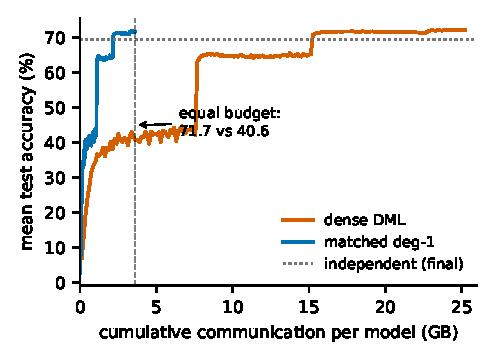
\includegraphics[width=\columnwidth]{figures/pareto.pdf}
\caption{Accuracy versus cumulative per-model communication (ResNet-32
$\times 8$, clean). Dense DML spends bandwidth $7\times$ faster for a final
premium of $+0.4$ points; at the budget where the single-partner cohort
converges (3.6\,GB, 71.7\%), dense has reached epoch 28 and 40.6\%---below
even the independent floor.}
\label{fig:pareto}
\end{figure}

\begin{table}[t]
\centering\small
\caption{The degree ladder at $K{=}12$ (mean over 5 seeds; ``share'' is the
fraction of the dense benefit over independent). The same ladder under 40\%
label noise shows the conversion effect and the same saturation.}
\label{tab:ladder}
\begin{tabular}{lccccc}
\toprule
 & & \multicolumn{2}{c}{clean} & \multicolumn{2}{c}{40\% noise}\\
arm & deg & acc & share & acc & share\\
\midrule
independent      & 0  & 69.51 & --    & 50.63 & -- \\
matched-1 (rand) & 1  & 71.72 & 84\%  & 58.34 & 90\% \\
fixed ring       & 2  & 71.52 & 76\%  & 58.49 & 92\% \\
matched-2        & 2  & 71.74 & 84\%  & 58.61 & 93\% \\
prism (fixed)    & 3  & 71.88 & 90\%  & 58.59$^{\dagger}$ & 93\% \\
random 3-reg.\ (fixed) & 3 & 71.90 & 91\% & 58.67 & 94\% \\
dense            & 11 & 72.15 & 100\% & 59.22 & 100\% \\
\bottomrule
\multicolumn{6}{l}{\scriptsize $^{\dagger}$healthy-model mean; one run
contained a spontaneously}\\[-2pt]
\multicolumn{6}{l}{\scriptsize collapsed member (\S\ref{sec:failure}).}
\end{tabular}
\end{table}

Table~\ref{tab:ladder} gives the central result at $K{=}12$; the same
pattern holds at $K=4$ and $8$ and in heterogeneous cohorts. Three features
recur everywhere. (i)~The first unit of degree buys most of the benefit:
degree~1 captures 84\% clean and 90\% under noise. (ii)~Returns diminish
smoothly; the dense premium is real (paired $p<0.05$) but costs $K{-}1$
messages per model per round against degree-1's single message. (iii)~Across
cohort sizes the dense premium grows slowly ($+0.29/+0.38/+0.48$ at
$K{=}4/8/12$) while its relative cost explodes ($3\times/7\times/11\times$);
matched-1 accuracy saturates by $K{=}4$. The cohort-size gains reported for
dense DML are, in our data, almost entirely a degree effect.

\textbf{Iso-communication.} Fig.~\ref{fig:pareto} makes the budgeted
comparison explicit: $+31.0$ points for sparse at equal bytes. Dense's final
half-point costs sevenfold bandwidth---a trade essentially every distributed
deployment declines.

\begin{figure}[t]
\centering
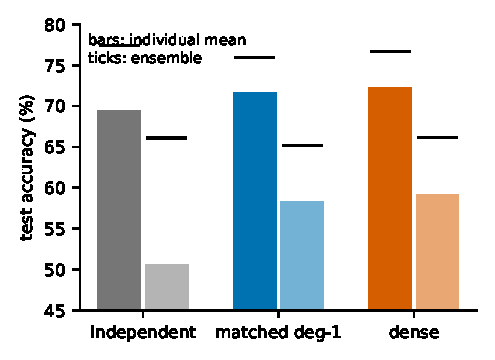
\includegraphics[width=\columnwidth]{figures/conversion.pdf}
\caption{The conversion mechanism ($K{=}12$). Bars: mean individual
accuracy; ticks: ensemble. Under noise, independent individuals collapse
(50.6) while their ensemble holds 64.8; any coupling converts collective
knowledge into individual competence, at a cost to the ensemble itself.}
\label{fig:conversion}
\end{figure}

\begin{table}[t]
\centering\small
\caption{Dataset transfer (CIFAR-10, ResNet-32 $\times 8$, 5 seeds): the
ordering, both nulls, and the conversion effect replicate. Under noise the
single random partner recovers the \emph{entire} dense benefit at $1/7$ the
communication.}
\label{tab:transfer}
\begin{tabular}{lcccc}
\toprule
 & \multicolumn{2}{c}{clean} & \multicolumn{2}{c}{40\% noise}\\
arm & acc & ens & acc & ens\\
\midrule
independent & 92.61 & 94.63 & 72.38 & 86.79\\
random-1    & 92.86 & 94.31 & \textbf{82.63} & 88.39\\
MWM-1       & 93.02 & 94.36 & 82.39 & 88.26\\
dense       & 93.16 & 94.47 & 82.16$^{\dagger}$ & 88.21\\
\bottomrule
\multicolumn{5}{l}{\scriptsize $^{\dagger}$healthy-model mean; one run
contained three spontaneously}\\[-2pt]
\multicolumn{5}{l}{\scriptsize collapsed members with no contagion
(\S\ref{sec:failure}).}
\end{tabular}
\end{table}

\textbf{Dataset transfer.} Table~\ref{tab:transfer} repeats the headline
cell on CIFAR-10. Every qualitative claim replicates: the ordering
(independent $<$ sparse $\approx$ sparse $<$ dense), the selection null
(MWM $-$ random $= +0.12$ clean, $-0.24$ noise), and the ensemble trade-off
(independent ensembles on top). Clean-tier magnitudes compress with the
reduced headroom near the 93\% ceiling (dense benefit $+0.55$); the noise
tier carries the magnitude story, where conversion is \emph{larger} than on
CIFAR-100 ($+9.8$ to $+10.3$ points, fuel gap 14.4 vs 14.2) and the single
random partner recovers the entire dense benefit ($82.63$ vs
$82.16$--$82.50$)---the sharpest single datapoint for the communication
claim in the study.

\textbf{Why coupling helps: conversion.} The noise cell
(Fig.~\ref{fig:conversion}) exposes the mechanism. Independent training under
40\% label noise leaves individuals at 50.6\% while their ensemble attains
64.8\%---the cohort knows collectively what no member knows individually,
because members err diversely. Coupling converts this collective surplus
into individual competence, compressing the ensemble--individual gap from 14
to $\approx$6 points; degree~1 performs 90\% of the conversion. The
conversion is paid for in diversity: every coupled ensemble sits below the
independent ensemble (76--77 vs 77.4 clean), a cost we report rather than
hide, and the reason two-phase ensemble distillation retains a niche sparse
online coupling cannot fill.

\section{Nothing Else Matters}
\label{sec:nulls}

\begin{table}[t]
\centering\small
\caption{The null ledger: every structural refinement of \emph{who} to
imitate ties its unstructured control (representative cells; full tables in
the appendix). $\Delta$ is the paired difference, $+$ favoring the
refinement.}
\label{tab:nulls}
\begin{tabular}{llc}
\toprule
refinement vs.\ control & cell & $\Delta$ (pp)\\
\midrule
MWM(disagreement) vs random     & $K{=}8$ clean  & $+0.21\ (p{=}.08)$\\
MWM(disagreement) vs random     & $K{=}8$ hetero & $-0.25\ (p{=}.21)$\\
MWM(per-class) vs random        & $K{=}8$ clean  & $+0.05\ (p{=}.71)$\\
MWM(teachable) vs random        & hetero         & $-0.11\ (p{=}.58)$\\
frozen vs rotating partners     & $K{=}8$ hetero & $+0.00\ (p{=}.99)$\\
DML$_e$ (avg.\ target) vs DML   & $K{=}8$ clean  & $-0.06\ (p{=}.74)$\\
prism vs expander (deg.\ 3)     & $K{=}12$ clean & $-0.04\ (p{=}.87)$\\
ring vs matched-2 (deg.\ 2)     & $K{=}12$ clean & $-0.22\ (p{=}.13)$\\
isolated 4-cliques vs prism     & $K{=}12$ clean & $-0.12\ (p{=}.21)$\\
isolated pairs vs matched-1     & $K{=}12$ clean & $\mathbf{-0.46\ (p{=}.008)}$\\
\bottomrule
\end{tabular}
\end{table}

Table~\ref{tab:nulls} summarizes the ablation program. Four selection
signals, rotation schedules, target composition, teacher weighting, and
graph shape at fixed degree all tie their controls; the marginal
clean-cell MWM effect ($+0.21$, $p{=}0.08$) is the largest selection signal
we ever observed and is worth at most a fifth of a point.

The one significant row is the most informative. Fully \emph{disconnected}
sub-cohorts---the strongest possible violation of connectivity---match their
connected counterparts almost exactly: isolated $m$-cliques land within
0.06~points of the value predicted by treating them as independent
$K{=}m$ cohorts (pairs: 71.26 vs 71.20 predicted; 4-cliques: 71.76 vs
71.72). Connectivity's entire measurable value is \emph{local pool access}:
being locked to one partner forever costs $-0.46$ relative to rotating over
eleven ($p{=}0.008$), and this pool premium is already inside noise by pool
size~3. No transport component is detectable---under clean or noisy
training, at any capacity we tested. We attempted to amplify structure
effects with the largest competence gradients available (40\% noise) and
with weak learners; the same-degree spreads did not widen.

We offer an explanation rather than a mere tally: with fully shared data
there is no knowledge \emph{gradient} between models, and a communication
graph with nothing to transport is invisible; only the local exchange rate
(degree) and the local pool remain. This predicts where structure should
re-enter: wherever a strong gradient exists. The next section confirms the
prediction in an unexpected channel.

\section{The Failure Channel}
\label{sec:failure}

\begin{figure}[t]
\centering
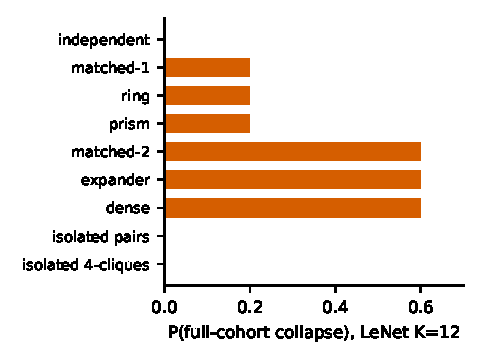
\includegraphics[width=\columnwidth]{figures/contagion.pdf}
\caption{Fragile cohorts (LeNet, $K{=}12$): probability that one spontaneous
single-model collapse cascades to the full cohort, by communication
pattern. Disconnected topologies (green) never propagate across a
boundary; deaths inside a clique remain inside it.}
\label{fig:contagion}
\end{figure}

\begin{figure*}[t]
\centering
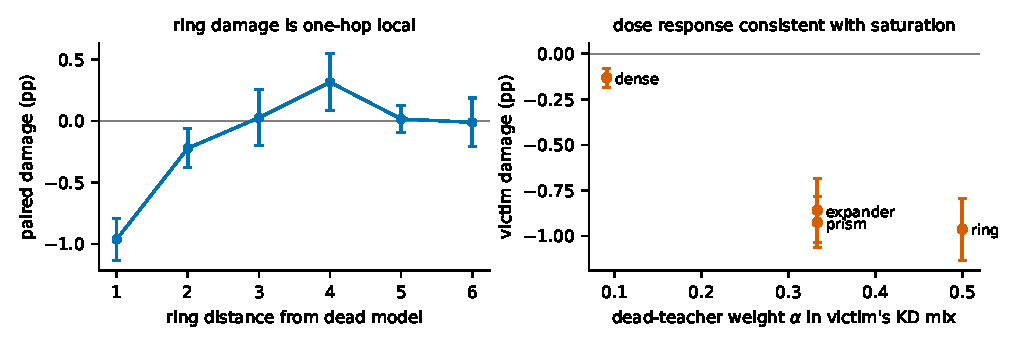
\includegraphics[width=0.9\textwidth]{figures/damage.pdf}
\caption{Robust cohorts (ResNet-32, $K{=}12$) with one implanted dead model
(frozen uniform-output teacher), all comparisons paired per-model against
bit-identical no-implant runs. Left: damage by ring distance---significant
at distance 1 ($-0.96$, $p{<}10^{-3}$), absent beyond. Right: chronic
dose--response across arms; damage saturates above teacher weight
$\alpha\approx 1/3$ and dilutes to $-0.13$ at dense's $\alpha=1/11$.}
\label{fig:damage}
\end{figure*}

A mutual-learning link is bidirectional: it carries whatever the peer
emits, including failure. We characterize this channel in both host regimes.

\textbf{Contagious collapse (fragile hosts).} LeNet cohorts exhibit rare
spontaneous single-model collapse under the shared recipe ($\approx$7\% of
models, an optimization fragility present even without communication). With
communication, a collapsed model---which emits near-uniform predictions---can
kill its neighbors, who then emit uniform predictions in turn: full-cohort
collapse occurred in 12/30 connected coupled runs versus 0/5 independent and
0/10 disconnected (Fig.~\ref{fig:contagion}). The infection respects graph
structure precisely: it never once crossed a clique boundary, and its
traversal time tracks mixing (10 epochs around the ring; 3 across the
expander; 2 under rotation). Notably, the survivors gained nothing:
at this capacity coupling has no constructive benefit either.

\textbf{Dose--response and healing (robust hosts).} To turn the accident
into a law, we implant one permanent dead model (frozen, exactly-uniform
logits---the fixed point a collapsed model approaches) in otherwise-healthy
ResNet-32 cohorts, across seven communication patterns, with healthy slots
initialized identically to no-implant anchor runs (35 runs). Results
(Fig.~\ref{fig:damage}): direct neighbors lose $0.9$--$1.0$ points under
chronic exposure at $\alpha\ge 1/3$, saturating in $\alpha$ and diluting to
$-0.13$ at dense's $\alpha=1/11$; second-hop damage is $\approx-0.2$ to
$-0.3$ where measurable and zero at three hops; partitioning quarantines
exactly ($+0.03$ outside the sealed clique); and \emph{no healthy model died
in any run}: victims degrade but remain informative teachers, so the chain
stops---the fragile-host epidemic requires susceptible hosts. Under rotation
the exposure is pulsed, and the damage \emph{heals}: models whose last
contact was within 10 epochs carry $-0.69$, while those with 11--30 epochs
of recovery are statistically unharmed (recency--damage correlation
$r{=}0.29$, $p{=}0.03$). A member of a sealed clique pays a compound price
($-1.22$): the chronic dose plus the loss of one live pool member, the two
independently-measured effects summing correctly.

\textbf{Design consequence.} The safest protocol \emph{inverts} with host
robustness. For robust cohorts, rotation is safest: exposure is spread thin
and heals (net damage $\approx 0$ at $k{=}2$), while fixed sparse graphs
make neighbor damage permanent and dense exposes everyone. For fragile
cohorts the ordering flips: rotation was the fastest contagion vector, and
partition the only reliable safety. Fault-tolerant cohort design thus
depends on which side of the susceptibility threshold the members sit---and
communication structure, inert for accuracy, is the control variable for
risk.

\section{Discussion and Limitations}

\textbf{When does this matter?} Absolute logit traffic is modest; the
communication argument binds in decentralized and edge settings, at large
$K$, or wherever the coupling must cross a network. The fault-tolerance
argument binds anywhere a member can silently degrade---which is everywhere.

\textbf{Limitations.} Our evidence base is CIFAR-scale classification under
a single training recipe (the CIFAR-10 transfer grid of
Table~\ref{tab:transfer} being the second dataset); the fragile-host collapse is recipe-dependent
(warmup would likely mute patient zero, though not the propagation law it
revealed); capacity and stability are confounded in the LeNet probe; and the
per-cell effects that separate structured alternatives are tenths of a
point, so our nulls are statements of practical, not metaphysical,
equivalence. Finally, our setting shares all data among members; in
partial-information regimes---sharded supervision, rationed
oracles~\citep{beikihassan2023resource}---knowledge gradients exist for
structure to transport, and we conjecture (with preliminary support from the
gradient-coupling account above) that selection and topology re-activate
there. Mapping that crossover is the natural next campaign.

\textbf{Conclusion.} Mutual learning needs linear, not quadratic,
communication; its benefit is a local, dose-controlled conversion of
collective diversity into individual competence, indifferent to who talks to
whom; and the structure of the communication graph, irrelevant to what a
cohort learns, decides how it fails.

\bibliographystyle{plainnat}
\bibliography{refs}

\end{document}
